\section{Data Cleaning Survey}
Between April 2015 and Dec 2015, we conducted two surveys and interviews with engineers, data analysts, and scientists who self-reported that they directly work with data in their organizations (N=29).

\subsection{Methods}
The surveys consisted of a series of quantitative questions about tool/language preference and job description, and several open-ended questions about the participants' organization's data management challenges. The interviews mirrored the surveys and were conducted and recorded. It is important to note that we conducted two separate surveys to ensure that our survey questions were properly calibrated. The first survey was conducted in June 2015, and we collected 5 responses to a preliminary set of 18 questions, and we conducted 4 in-person/phone interviews based on the same questions. Using the results of this survey, and revising the questions, we conducted a second survey with more specific language on the questions that received 21 participants. 
Most of the participants were contacted personally by the authors and were often acquaintances of the authors. However, the authors took care to ensure that the participants were not informed of any of the quantitative hypotheses or conclusions of the study before taking the survey. 
Some participants were reached through forums frequented by data analysts\footnote{http://reddit.com/r/datascience}, and all participants had the option to take the survey anonymously.

The questions and the data for the survey are available at: \url{http://TODO}

\subsubsection{Participant Demographics}
The survey asked a series of questions about the participants' job descriptions, expertise, and use of certain tools/interfaces.
We briefly summarize the results.

\vspace{0.5em}

\noindent\textbf{Job Descriptions: } We requested participants to provide a job description and details about their organizations. We categorized the participants by their reported organization size and their roles. The participants were mostly from larger organizations (defined as > 100 employees). We also found that they were mostly evenly split between infrastructure and data analytics. A surprisingly larger number (7/30) reported that they performed both roles in their organizations. The results are summarized in Table \ref{tab:jobs}. 

\begin{table}[t]
\centering
\begin{tabular}{|l|r|}
\hline
Size                               & Number \\
\hline
Small    & 7      \\
\hline
Large & 17     \\
\hline
N/A                                & 5\\  \hline  
\end{tabular}
\quad
\begin{tabular}{|l|r|}
\hline
Job Desc.                              & Number \\
\hline
Infrastructure    & 10      \\
\hline
Analysis & 12     \\
\hline
Both                                & 7\\  \hline  
\end{tabular}

\caption{Categorized responses to the question ``Describe your company/organization and your role there.'' We defined a large organization as one with > 100 employees. To determine the job description, there was a clarifying question ``I develop infrastructure to process incoming and historical data at scale for use by other business units.". \label{tab:jobs}}
\end{table}

\vspace{0.5em}
\noindent\textbf{Data Products: } Machine Learning is an increasingly popular use-case for large datasets. We asked participants who self-reported as data analysts whether they work with Machine Learning. We found that 11/17 ``data analyst'' participants reported working with machine learning models.

\vspace{0.5em}
\noindent\textbf{Tools/Interfaces For Cleaning: } Next, we asked participants about the existing tools and interfaces they used for data cleaning. This set of questions was only asked in the second survey. Figure \ref{fig:interfaces} shows the results. We find that most of the participants responded that they used Python/Perl or MapReduce-like frameworks (clarified in the survey to be Spark/Hadoop etc.) to manipulate data before analysis. A minority of participants responded that they used graphical interfaces or rule-based interfaces to clean data.

\begin{figure}[t]
\centering
 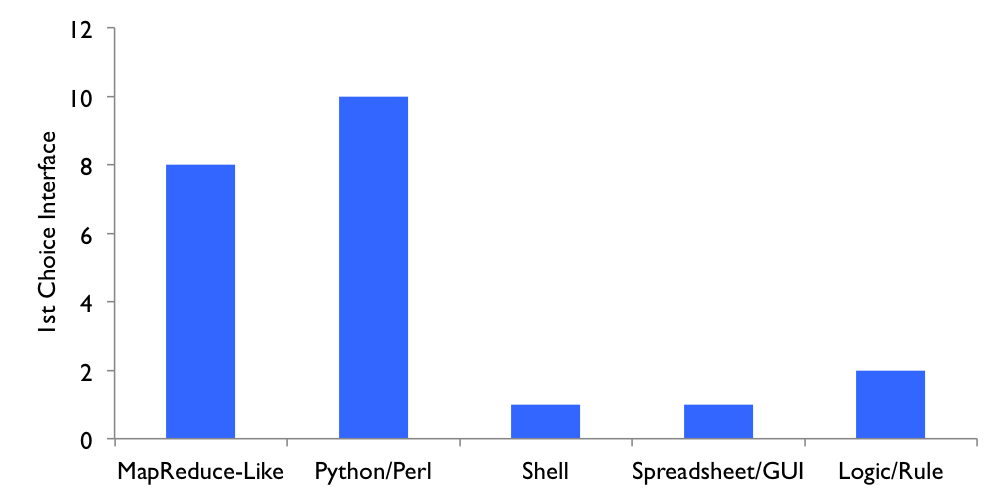
\includegraphics[width=\columnwidth]{datafigs/hilda-interface.png}
 \caption{Top ranked responses to: ``Which of the following tools/interfaces/languages do data scientists at your organization prefer for manipulating data, including extraction, schema transformations, and outlier removal, to make analysis easier or more reliable. Please Rank.''\label{fig:interfaces}}
\end{figure}


\subsection{Themes}
We highlight several of the themes we discovered from the survey and the interviews: (1) the tension between infrastructure engineers and data analysts, (2) debugging and validation in data cleaning, and (3) methodology and over-fitting.

\subsubsection{Analysts vs. Infrastructure}
As noted by our demographics analysis, there are three main segments of data engineers: analysts, infrastructure engineers, and those who do both.
One of the most important themes that we discovered in the data was the divide between infrastructure engineers and analysts in how these groups address data quality problems. In particular, we see a difference in the way that these two groups of participants conceptualize dirty data, the solutions, and repair procedures.

One of the most significant tensions between the infrastructure engineers and analysts is about the definition of dirty data. While the infrastructure engineers are in charge of the data ingest pipelines, ETL, and other pre-processing steps, it is often the analysts who get to ``define'' what is dirty. One infrastructure engineer noted the frustration about being caught in the middle between the business units that generated the data and the analysts querying the data:

\vspace{0.5em}
\emph{There are often long back and forths with senior data scientists, devs, and the business units that provided the data on data quality. It is almost never a smooth process. The vast majority of problems are in turning semi-structured data into features. What placeholder value is sensible to use for a missing value, do we replace it with the mean or nearest neighbor; or is a variable ordinal or categorical? These are tough questions that often can only be answered by the business unit themselves. We try to get them to do some of this work but it inevitably falls on us esp. if it is a big unit.}

\vspace{0.5em}

The tension between the infrastructure engineers and the data analysts seems to stem from the semantics of data and who knows these semantics. Our responses also suggest that the definition of data error is highly analysis dependent. In response to how she defines dirty data, one analyst responded

\vspace{0.5em}
\emph{Domain expertise, I guess. I wish there were a more rigorous way to do this but we look at the models and guess if the data are correct. -Analyst}



Furthermore, we see a distinct difference in concerns for these two groups. For the infrastructure engineers, we found that most saw dirty data as symptomatic of an error in the processing pipeline (i.e., a software bug or incorrect schema). Their goal was to rectify the bug or drop the corrupted data with a minimal impact on system SLOs:

\vspace{0.5em}
\emph{There are software bugs in the application such as edge cases that are not handled or changes to the services by programmers that have unintended consequences. Fixing data errors in a high-availability setting is challenge as it may require shutting of services. -Infrastructure Engineer}

\vspace{0.5em}

Most of the infrastructure engineers surveyed used sampling or unit testing to detect obvious problems in the data processing pipeline.

\vspace{0.5em}
\emph{We have checks for file consistency, if the end of files look like the write was interrupted early, whether the size of a file seems significantly bigger or smaller than usual, etc. we check data with some standard queries to make sure the files have the expected range of values, ie for every country, and every minute of the day there was data. -Infrastructure Engineer}

\vspace{0.5em}

Based on the infrastructure engineers' responses, it would seem like there are relatively straight-forward and efficient techniques for ``cleaning'' data. However, the data analysts disagreed. The data analysts were less concerned about obvious problems in extraction and more concerned about subtle errors invalidating their analysis or biasing their machine learning models. One analyst said,

\vspace{0.5em}
\emph{Most of these errors are subtle enough that the analysis will go through e.g., with standard null value semantics of SQL, but give an incorrect answer. Usually is only caught weeks later after someone notices something like...well the Wilmington branch cannot have 1M sales in a week}

\vspace{0.5em}



  

How do we detect dirty data?

How do we deal with dirty data?: 

Is Dirty Data Too Big?: To both groups of participants we asked the question “Has the scale of the data ever made it challenging to clean”. (k/N) We found that most of the self-reported infrastructure engineers suggested that scale was NOT an issue, while we found that (k/N) the reverse was true among the data analysts. This suggests that the type of dirty data is important to the question of scale. Errors that are semantic in nature may be harder to clean and detect as they require more discretion from the analysis.

“Build around common formats, otherwise it's all domain- and content-specific. Without fail, a non-trivial effort is required to "reduce problem to one previously solved", whether it be data access or translation of format for use with pre-existing tools.”-Infrastructure Engineer

“We usually do not do rigorous validation of data cleaning. We typically clean our data until the desired analytics works without error. This is not desirable but practical since in most cases data error is probably overshadowed by errors/inaccuracies in the models themselves.” -Data Analyst

.

Iteration vs. Interactiveness

“Do your level best on initial sample of data, determine what are exceptions and build filters. Iterate with greater knowledge.”

“Iterative process, where I assess biggest problem, devise a fix, re-evaluate. It is dirty work.”

“Usually the most time is spent getting the data into a state where your code even runs. After that, we make sure that we can explain every trend seen in the analysis.”

Semantics of the data and who knows it

“Domain expertise, I guess. I wish there were a more rigorous way to do this but we look at the models and guess if the data are correct.”

“When records are dirty, we usually identify the source of truth (in our case a hospital) and call them and figure out what is going on.”

“Much of the data cleaning and formatting logic goes into design views of the data that exclude errors or particularly questionable data. We design such processed data views with the help of development operations. Of course there are times when we have to go back to the source data to figure out if there are any artifacts in our analysis.”





Interactive vs noninteractive

How does debugging/validating correct cleaning get done?

The 99 percent

Overfitting the cleaning
